\documentclass{article}
\usepackage{graphicx}
\usepackage{amsmath}
%\usepackage[scientific-notation=true]{siunitx}
\usepackage{tabularx}
\newcommand{\D}{\displaystyle}
\begin{document}

\title{Inferring Characteristics of Interaction Matrices in an Ecological Context{}}
\author{Naika Dorilas}

\maketitle

\begin{abstract}
In ecology, an interaction matrix describes how species in an ecosystem interact with one another and affect each others growth in a given model of population growth. In an attempt to find a method for inferring species interactions, many ecologists have tried to go from time series data on the population fluctuations of species to inferring the entire interaction matrix. In this paper, the objective is to infer parameters of the interaction matrix, given a set of data, so instead of inferring the entire matrix, we just want 3 key statistical properties about how the entries are drawn, the mean $\mu$, variance $\sigma$ and average diagonal elements d. So based on a specified ecosystem we are trying to find a method of inferring the statistical properties of the interaction matrix between different species based on a simple model of population fluctuation. We will use maximum likelihood, to predict the probability of observing our data, x given $\mu, \sigma, d$. So what we expect from this maximization are the $\mu,\sigma,d$ that make the data, or fluctuations in population sizes of the species the most likely. The implications of this are that assuming this method is successful, any randomly generated matrix with the given statistical properties found could be used to describe how species in the data set used interact.
\end{abstract}

\section{Background}

\subsection{What is random matrix theory?}
\hfill\break
Random Matrix Theory is a combination of statistics and traditional matrix theory. In this field, many tools from statitistics are used to describe matrices with random elements instead of relying on those individual elements. It allows us to generalize about certain characteristics of mtrices with similar statistical properties. Many problems in physical systems modeling and biological systems modeling involve matrices with random entries. \hfill\break

Random matrix theory has some great uses for the context of this project. Traditionally in one-dimensional models of population growth, specifically Lotka Volterra there are birth rates $r_b$, death rates $r_d$, and a carrying capacity, K.  \hfill\break
\hfill\break 
$$
N(t+\Delta t)=N(t)+\Delta t (r_b-r_d)N(t)(1-\dfrac{N(t)}{K})
$$
\hfill\break \hfill\break
Although, if we want to include the effects of other species on a single species, in ecological models of population growth across species we need to include something called an interaction matrix. It describes the way that different species interact with each other and effect eachothers survivial whether it be positively, negatively or with no effect at all. If we look at the equilibrium solutions-which tells us about stability of systems-and take them in smal perturbations, we get this linearized model of population dynamics \hfill\break
\hfill\break 
\begin{equation}
y_i(t+\Delta t)=y_i(t) + \Delta t(A_{ij}y_i +\xi_i)
\end{equation}

\hfill\break
where $y_i(t)$ is the population of species i at time t, $\xi_i$ is random noise that might affect a species growth, and $A_{ij}$ is the matrix that describes the interactions between the species.
\hfill\break 
If we subtract both sides by $y_i(t)$, divide by $\Delta t$ then allow $\Delta t \rightarrow 0$ then we obtain \hfill\break
$\dfrac{\partial y_i}{\partial t}=A_{ij}y_i$
we also dropped the random noise variable in order to illustrate species interactions simply.
\subsection{Examples of Interaction Matrices}

An example interaction matrix is illustrated below. 

$$
\begin{bmatrix}
x_{11}&x_{12} \\
x_{21}&x_{22}
\end{bmatrix}
$$
\hfill\break \hfill\break
Here we have a small ecosystem of just 2 species for simplicity. In this case the model for population size of species i can be expanded to, 
\hfill\break
\hfill\break
\begin{equation}
\begin{cases}
\dfrac{dy_1}{dt}=x_{11}y_1+x_{12}y_2\\\\
\dfrac{dy_2}{dt}=x_{21}y_1+x_{22}y_2\\\\
\end{cases}
\end{equation}
\hfill\break
\hfill\break
Now we will explore a couple of different cases of what could happen when two species interact with eachother and what this looks like in terms of the interaction matrix and the model.
\hfill\break
\hfill\break
\textbf{Example 1:}\hfill\break
\hfill\break
We could have a situation where the interaction matrix looks as such \hfill\break
$$
\begin{bmatrix}
x_{11}&0 \\
0&x_{22} 
\end{bmatrix}
$$
In this case, the off diagonal elements are equal to 0, if we expand model (1) for this interaction matrix we get:
\begin{equation}
\begin{cases}
\dfrac{dy_1}{dt}=x_{11}y_1\\\\
\dfrac{dy_2}{dt}=x_{22}y_2\\\\
\end{cases}
\end{equation}
Now we can see that the population of species 2 does not appear in the dynamics for species one and vice versa meaning the species are not interacting at all.\hfill\break\hfill\break\hfill\break
\textbf{Example 2:} \hfill\break\hfill\break
We could also have a case where the interaction matrix looks like this:
$$
\begin{bmatrix}
x_{11}&0 \\
x_{21}&x_{22} 
\end{bmatrix}
$$
In this case if we exapand the equations in model (1) we would get something like this:
\begin{equation}
\begin{cases}
\dfrac{dy_1}{dt}=x_{11}y_1\\\\
\dfrac{dy_2}{dt}=x_{21}y1+x_{22}y_2\\\\
\end{cases}
\end{equation}
meaning that species 2 has no effect on the population dynamics for species 1 but species 1 is postively benifiting the populaiton of species 2. This could happen in a case of commensalism where species 1 is not being harmed or helped by species 2 but species 2 is gaining something from interacting with species 1.
\hfill\break\hfill\break\hfill\break

\textbf{Example 3:} \hfill\break\hfill\break
In this case we have an interaction matrix that looks like this

$$
\begin{bmatrix}
x_{11}&-x_{12} \\
x_{21}&x_{22} 
\end{bmatrix}
$$
\hfill\break
and if we expand model (1) we have something that looks like this:
\begin{equation}
\begin{cases}
\dfrac{dy_1}{dt}=x_{11}y_1\\\\
\dfrac{dy_2}{dt}=x_{21}y_1+x_{22}y_2\\\\
\end{cases}
\end{equation}
This shows us that species 2 is having a negative effect on the dynamics of species one and that species one is having a positive effect on the dynamics of species 2. An instance where this could happen is if there is a parasitic relationship between the two species or predation.
\hfill\break
\subsection{The Need For Larger Matrices}
\hfill\break
Now this is what happens in a two-dimensional case, if we make the interaction matrix larger, the same kinds of patterns for different entries follow.\hfill\break
$$
\begin{bmatrix}
   x_{11} & x_{12} & x_{13} & \dots &x_{1, 100}&\dots & x_{1n} \\
    x_{21} & x_{22} & x_{23} & \dots &x_{2,100}&\dots & x_{2n} \\
    \vdots & \vdots & \vdots & \ddots & \vdots &\vdots&\vdots \\
x_{100,1}&x_{100,2}&x_{100,3} &\dots & x_{100,100}&\dots& x_{100,n}\\ 
\vdots & \vdots& \vdots& \vdots& \vdots &\ddots&\vdots \\
    x_{n1} & x_{n2} & x_{n3} & \dots &x_{n,100}&\dots & x_{nn}
\end{bmatrix}
$$\hfill\break
In biological systems many aspects of the environment and growth process are random, large and can vary over space and time. For higher dimension interaction cases, the exact entries of the matrix matter less than certain aspects about the distribution of their entries such as the mean $\mu$, variance $\sigma$ and diagonal elements d. Random Matrix Theory(RMT) allows us to understand the stability of an ecosystem through looking at large scale properties of the matrix which we often refer to as an interaction matrix A. We can determine when a system will be stable based on these properties because we have results from RMT that for instance tell us about the distribution of eigenvalues for random matrices with similar statistical properties. Eigenvalues, tell us about the stability of our equilibrium solutions: whether or not starting close to that equilibrium will result in staying close to that equlibrium or diverging. In Ecology that tells us about a species survival. It would give researchers alot of insight if they were able to get basic aspects of matrices that allow for a stable ecosystem in a given population.   \hfill\break

In this project we start with a stable symmetrical matrix for which there are many useful properties from Random Matrix Theory. Given a set of data and our simple population model (1), our goal was to infer paramaters:$\mu,\sigma,d$ of a random interaction matrix A that would best fit the data. What this means is that based on an arbitrary real world data set of populations of different species across time, we hoped to infer the statistics of how the species in that data set interact with eachother.



\section{Methods}
\subsection{Maximum Likelihood}
\hfill\break
So again, given time series data on poulation fluctuaton for S different species and our simple population model (1), our goal was to infer paramaters:$\mu,\sigma,d$ of a random interaction matrix A that would best fit the data. to do that we needed to maximize $P(x|\mu,\sigma,d)$ where x represents discrete data points for each species, particularly N of them. Given a statistical model-$f(x)$ and parameters-$p_i:p_1,p_2,...,p_n$,  $P(x|\mu,\sigma,d)$ is the likelihood of observing the model input x given the parameters p1:pn. Then we maximize this likelihood so our output from maximum likelihood becomes the parameter values:$p_i$ that make the x, the most probable. In the context of this project, x is the data of population dynamics of S different speices. We also have paramteres $p_i={\mu,\sigma,d}$ which describe the statistical properties of a random interaction matrix, and the output from maximum likelihood gives us the $p_i$ which makes the population fluctuations most likely to happen. So it optimizes $p_i$ by finding the parameters $p_i$ of a random interaction matrix which make those interactions the most likely to produce the fluctuations at each time step for S species: $x^a$, where a is the index for the number of data points drawn from each species.
\hfill\break\hfill\break
In this paper we assume that each discrete data point, $x^a$ from the an arbitrary time series are independent. Therefore the average probability of observing the data points for one species ,$x^a$ given our parameters, $p_i$ for each species 1:S is just the multiplication of these probabilities \hfill\break\hfill\break $P(x_i^1|p_i)\times P(x_i^2|p_i) \times \dots \times P(x^a|p_i)\times \dots \times P(x_i^N|p_i)$
\begin{equation}
P(x|\mu,\sigma,d)=\int dA \prod_{a=1}^N P(x_i^a|A)\times P(A|\mu,\sigma,d)
\end{equation}
\hfill\break where N is the number of data points we collect for each species.
\hfill\break\hfill\break Then we assume 3 things
\hfill\break\hfill\break
1). $A_{ij}=\dfrac{\mu}{S} + B_{ij}, B_{ij}~N(0,\dfrac{\sigma^2}{S}\leftarrow A_{ij}~N(\dfrac{\mu}{S},\dfrac{\sigma^2}{S})$ \hfill\break
2). $A_{ii}=-d+\dfrac{\mu}{S}$ \hfill\break
3). $\dfrac{1}{S}\overline{logD}=\dfrac{1}{S}(log(d+\mu)+(S-1)\int d\lambda \dfrac{\sqrt{4\sigma^2-(\lambda+d)^2}}{2\pi\sigma}\times log\lambda$ \hfill\break\hfill\break
So that the parameters $\mu, \sigma, d$ can be solved for, we one assume that the off diagonal elements of A are drawn from a normal distribution of mean $\mu$ and variance $\sigma^2$, both sized down by S, and two assume that the diagonal elements of A are $-d+\dfrac{\mu}{S}$\hfill\break
We will justify why we do this below, but the determinants for large matrices are very similar, so to simplify our calculation we take the average determinant of A. The determinant of a matrix is given by the multiplication of eigenvalues. So the third assumption comes from the semircular law in Random Matrix Theory by physicicst Eugene Wigner in 1955. The distribution of eigenvalues for a symmetric matrix A whose entries were generated randomly and independently by a given distribution with mean:$ \mu$, variance: $\sigma$ and average diagonal elements: d, lie on a semicircle centered at d with diameter $2\sigma$. The distribution of eigenvalues therefore comes from the formula \hfill\break
$$
\dfrac{\sqrt{4\sigma^2-(\lambda+d)^2}}{2\pi\sigma}
$$
\hfill\break
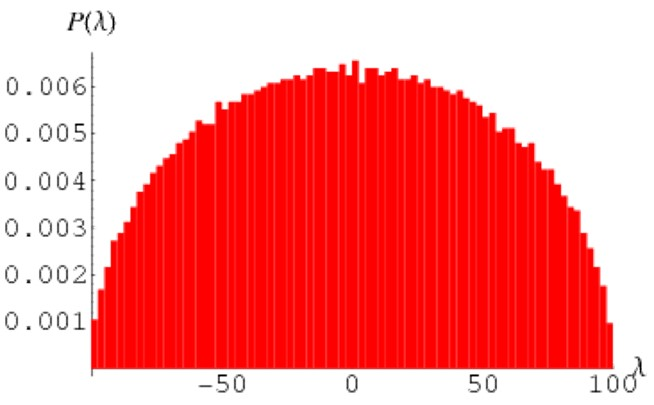
\includegraphics[scale=0.5]{Picture2} \cite{one}

\hfill\break\hfill\break

Now based on some of these assumptions 
$$
P(x|A)=\dfrac{(det(A))^{1/2}}{(2\pi)^{S/2}} exp(\dfrac{1}{2}\sum_{a=1}^N\sum_{ij}^S x_i^aA_{ij}x_j^a)
$$

We can then expand the likelihood equation to be 
$$
P(x|\mu,\sigma,d)=\int \prod_{i<j}^N(dA_{ij})\dfrac{(det(A))^{1/2}}{(2\pi)^{S/2}} exp(\dfrac{1}{2}\sum_{a=1}^N\sum_{ij}^S x_i^aA_{ij}x_j^a)\times P(A|\mu,\sigma,d)
$$
Since A is a symmetric $S\times S$ matrix for our purposes, then we only need to integrate over the upper right half of A. Then we just needed to multiply the $P(x|\mu,\sigma,d)$ for each $a \in$ [1,N]. \hfill\break \hfill\break So then after including our assumptions, since we are taking the average determinant of A we replace that term with D 
\hfill\break
\begin{equation}
\dfrac{2}{N}logP=logD-\dfrac{d}{N}\sum_{a}\sum_i (x_i^a)^2 +\dfrac{1}{SN}\sum_{a}(\sum_i x_i^a)^2+\dfrac{1}{2SN}\sum_{ab}(\sum_i x_i^a x_i^b)^2 
\end{equation}
gives us the simplified version of our log likelihood equations.
\hfill\break
Then we had to maximize this likelihood to obtain parameters $\mu,\sigma,d$. So we took the partial derivates with respect to each variable of the log likelihood and set them equal to 0. 
\hfill\break\hfill\break
$\dfrac{\partial logP}{\partial \mu}=0$,
$\dfrac{\partial logP}{\partial \sigma}=0$,
$\dfrac{\partial logP}{\partial d}=0$
\hfill\break
These equations based on the log likelihood can be written in the following form:
\begin{equation}
\begin{cases}
\dfrac{\partial D}{\partial \mu} \dfrac{1}{D}=-\dfrac{1}{SN}\sum_{a}(\sum_i x_i^a)^2 \\\\
\dfrac{\partial D}{\partial \sigma^2} \dfrac{1}{D}=-\dfrac{1}{2SN}\sum_{ab}(\sum_i x_i^a x_i^b)^2 \\\\
\dfrac{\partial D}{\partial d} \dfrac{1}{D}=\dfrac{1}{N}\sum_{a}\sum_i (x_i^a)^2 \\\\
\end{cases}
\end{equation}
Solving these systems of equations for $\mu,\sigma, d$ is the last step in completing this method.
\subsection{Simulating Data}\hfill\break
To ensure that our calculations were correct and that this method was valid we generated data from a multivariate normal distribution, 
$$P(x_i^a| A)=\dfrac{\sqrt{det(A)}^{N/2}}{2\pi^{NS/2}} exp(\dfrac{1}{2}\sum_{a=1}^N\sum_{ij}^S x_i^aA_{ij}x_j^a)$$ \hfill\break
Doing this, we assume X comes from discrete data points from each of S species. To make sure this method for inferring parameters is valid, we wanted to make sure it produces similar predictions for $\mu,\sigma,d$, as the $\mu,\sigma,d$ we gave to the simulation and used to generate the data. Given that our assumption of X is that it will come from this exact kind of distribution, our predicted values should closely match the actual values given to the simulation. An example of the time series data that we might take from each species is given in Figure 1. Where instead of taking all the data, we look at discrete time steps.
\hfill\break
\hfill\break
\hfill\break
\hfill\break
\hfill\break
\hfill\break
\hfill\break
\hfill\break
\hfill\break
\hfill\break
\begin{figure}
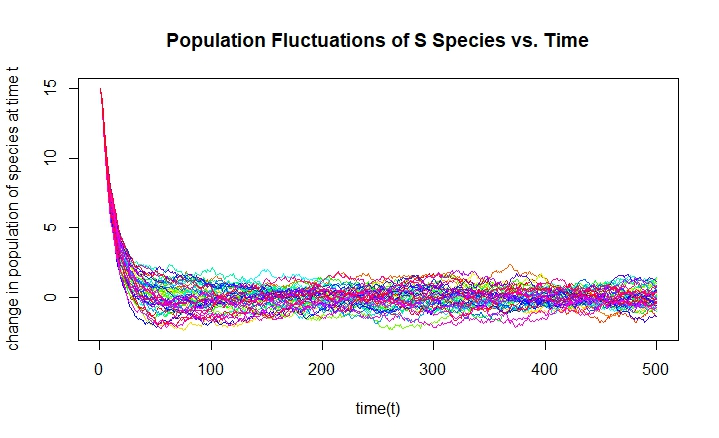
\includegraphics[scale=0.6]{Popf}
\end{figure}
\hfill\break
\hfill\break
\hfill\break
\hfill\break
\hfill\break
\hfill\break
\hfill\break
\section{Results}
\subsection{Validation of Methods}
To make sure his method was valid and can be applied to other uncorrelated data, we graphed the simulated log determinants vs the analytical log determinants , the Rhs vs Lhs of the maximization equations and the output our optimization function for different $\mu,\sigma,d$. What we wanted is \hfill\break\hfill\break 1) That the average log determinants of matrices made from different $\mu,\sigma,d$, to be close to the log determinants calculated from the semicircular law for those same $\mu,\sigma,d$. \hfill\break\hfill\break 2). We wanted the Lhs of the optimization equations that depend on $\mu,\sigma,d$ and the Rhs that depend on the data X, for different parameters that generate both sides to also be very close so that 
$\dfrac{\partial logP}{\partial \mu,\sigma,d}=Lhs-Rhs$=0. This is neccessary to be able to optimize for our parameters. \hfill\break\hfill\break 3). We wanted to see that the output for $\dfrac{\partial logP}{\partial\mu,\sigma,d}$ was equal to 0 at some point or else there would be no root and therefore no optimal $\mu,\sigma,d$. \hfill\break\hfill\break According to the following figures, 1), 2)., 3). were achieved.
\hfill\break
\hfill\break
1)\hfill\break
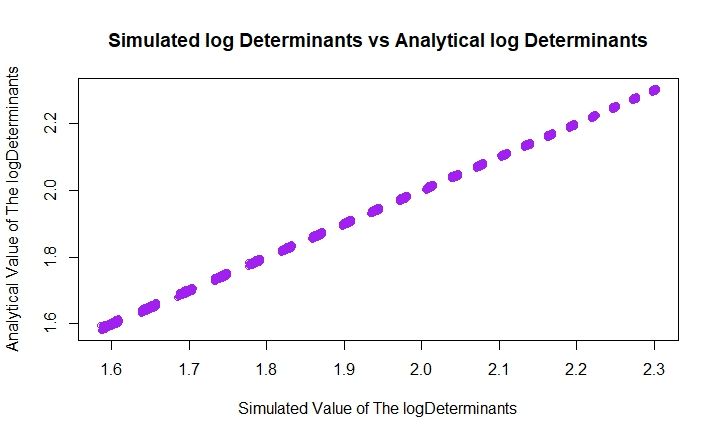
\includegraphics[scale=0.4]{LD}\hfill\break
2)\hfill\break
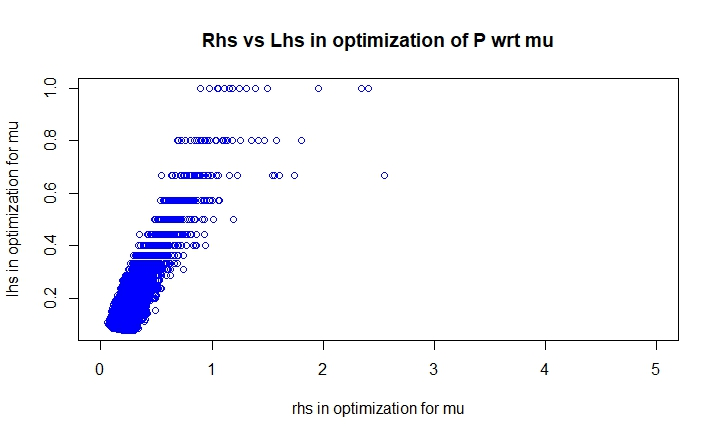
\includegraphics[scale=0.4]{rlmu}
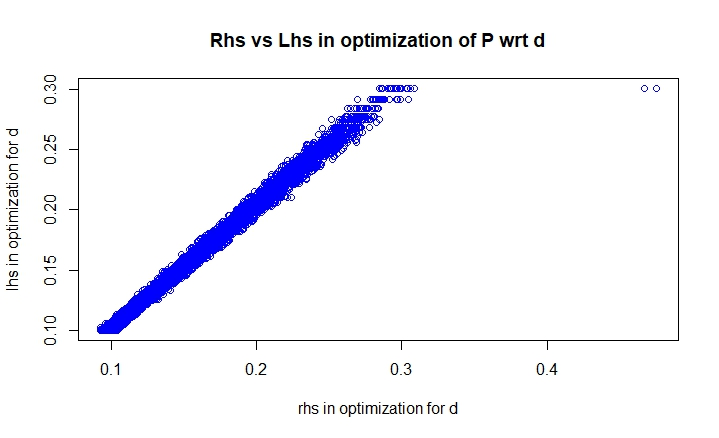
\includegraphics[scale=0.4]{rld}
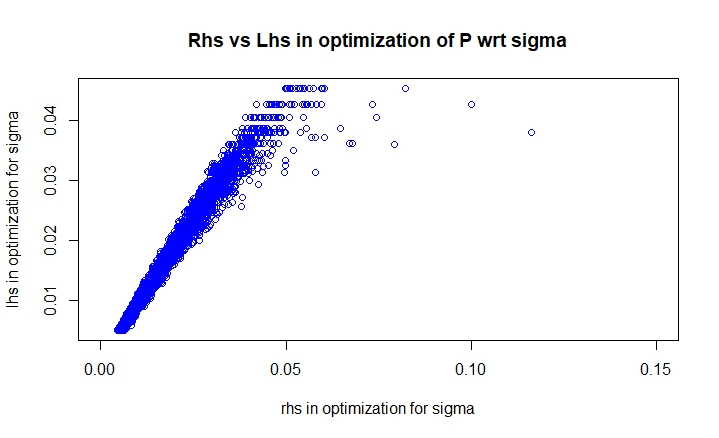
\includegraphics[scale=0.4]{rlsigma} \hfill\break
3)\hfill\break
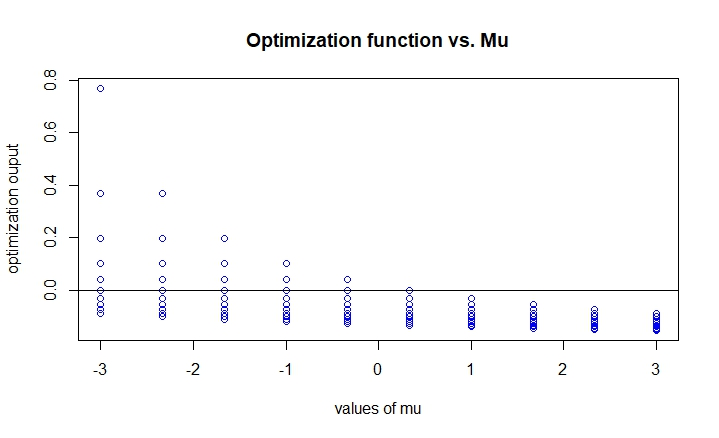
\includegraphics[scale=0.4]{OPmu}
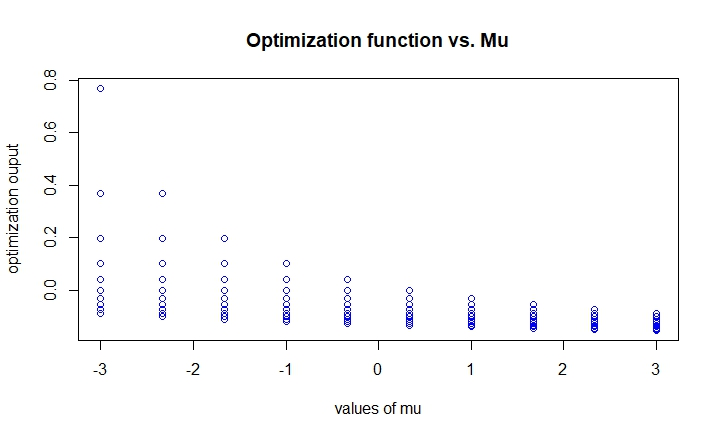
\includegraphics[scale=0.4]{OPsigma}
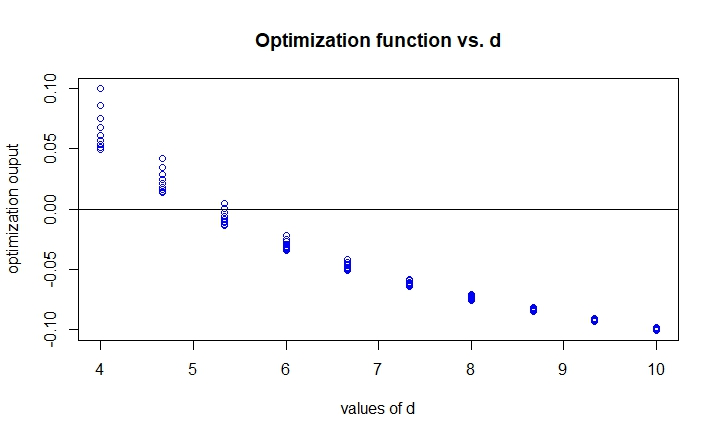
\includegraphics[scale=0.4]{OPd}

\subsection{Predicted output parameters vs actual parameters}\hfill\break
\hfill\break
As a result of technical difficulties for this project in terms of gaining valus for our estimations, we only plot The predicted values we obtained for d in comparison to the actual values for a number of iterations. 
\hfill\break
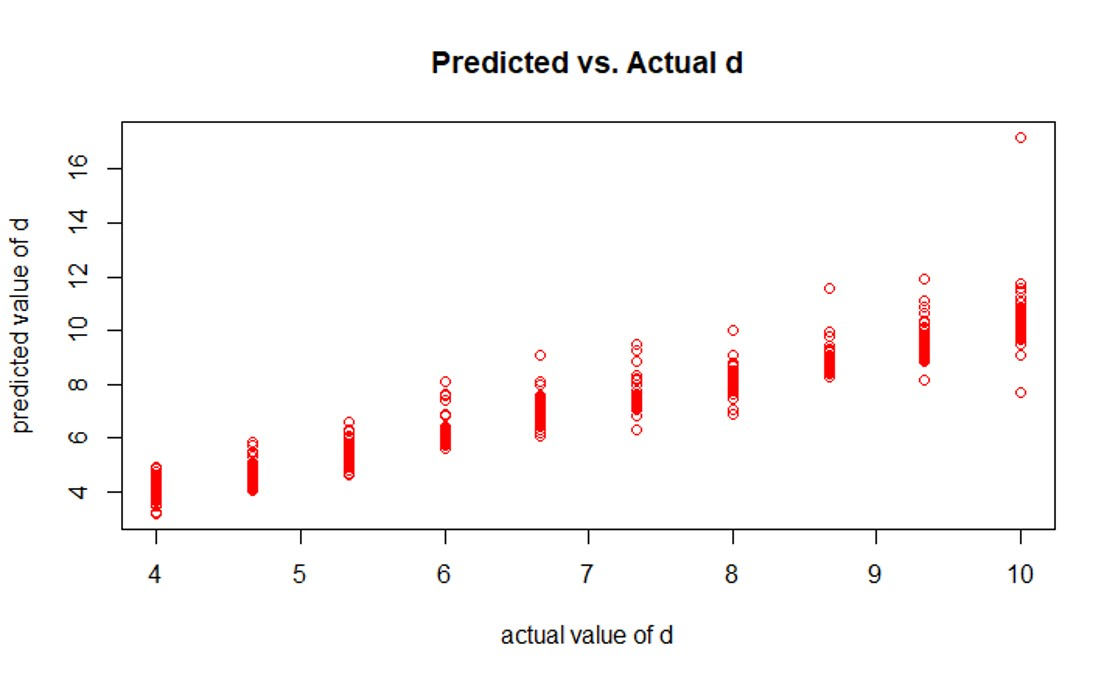
\includegraphics[scale=0.5]{Picture1}
%\begin{equation}
%\begin{cases}
%\dfrac{dT}{dt}=-\beta V T\\\\
%\dfrac{dI_1}{dt}=\beta V T- kI_1\\\\
%\dfrac{dI_2}{dt}= kI_1- \delta I_2\\\\
%\dfrac{dV}{dt}=\pi I_2- c V\\\\
%\end{cases}
%\end{equation}
%\hfill\break
\hfill\break
%\hfill\break
%\begin{table}
%\caption{Predicted Values of $\mu,\sigma,d$ in Comparison to the Actual Values of $\mu,\sigma,d$} 
%\centering 
%\begin{tabular}{lll}
%\hline
%Variable  & Predicted Value &Actual Value\\ [0.5ex]
%\hline
%\\
%&  &  $\D\frac{\mbox{}}{}$ \\ [0.5ex]	
%&  &  $\D\frac{\mbox{}}{}$ \\ [0.5ex]
%& &$\D\frac{\mbox{}}{}$ \\[0.5ex]
%& &  $\D\frac{\mbox{}}{}$  \\ [0.5ex]
%
%\hline
%\end{tabular}
%\label{table:variables} 
%\end{table}
%\hfill\break





\section{Discussion}
The impact of doing this method successfully is that hopefully we will be able to determine the key aspects of interaction given a specific data set and not have to infer an exact matrix. So we would be able to say that any random interaction matrix with those parameters $\mu, \sigma$ and d would be able to describe how the species in that given data set interact. I would soon like to see that this method still holds for $\mu, \sigma$ since d was the only estimation that currently works. Also, in the future I would like to use real world data sets of different species, and maybe even try multiple data sets and see how different types of data fare under this method. 

\hfill\break


\begin{thebibliography}{999}

\bibitem{one} Wigner's Semicircle Law. (n.d.). Retrieved from http://mathworld.wolfram.com/WignersSemicircleLaw.html

%On top of that, the stability of a biological system is very pertinent. In an ecological context it determines the survival of species. Generally we look at the "community matrix", which for a population of S species is influenced by S equations for population fluctuation. The community matrix looks at equilibrium solutions for these equations in small perturbations around the equilibria. We say the system is stable if when starting close to an equilibrium we stay close to that equilibria. Local stability can be determined by the eigenvalues of the matrix M. 

\end{thebibliography}
\end{document}